\section{Experiments}
\label{sec:experiments}
Every number below is read from files in \texttt{results/} produced by the shipped code (script map in \texttt{figures/SCRIPTS.md}; commands in \texttt{REPRODUCE.md}). Intervals over replicates are mean$\pm1.96\,$SE; coverage and decision rates carry Wilson 95\% intervals (T0); on the real matrix (T1) replicates share one item pool, so T1 intervals are delete-a-block.

\subsection{Synthetic world with exact truth (T0)}
\textbf{Design.} A latent-probit world: each configuration $c$ has a true accuracy $\theta_c=\Phi(a+\delta_c)$ with spread $\tau$ (SD of $\delta_c$ on the probit scale; $\tau=0$ means all configurations are equal), item difficulty is shared across configurations with latent correlation $\rho$ of configuration$\times$item effects, and outcomes are Bernoulli. Because $\theta(\hatc)$ is known exactly, bias and coverage are measured without noise on the truth. The grid covers $n\in\{50,\dots,2000\}$, $K\in\{2,\dots,200\}$ candidates, $\tau\in\{0,.05,.1,.2\}$, $\rho$, baseline accuracy, three search procedures (exhaustive, successive halving, greedy coordinate edit) and few-shot demonstrations drawn from $D$: 216 cells and 203{,}400 replicates (300--1000 per cell). The reference world is $\rho=0.6$, baseline accuracy 0.3, exhaustive search; the headline cells have 1000 replicates.

\textbf{How large is the gap, and what drives it?} (Fig.~\ref{fig:A}.) The naive report is optimistic in every cell with $K>1$ configurations compared. With $\tau=0$ (nothing to find) the mean optimism is 14.6 [14.2, 14.9] accuracy points at $n=50$, $K=200$, 4.5 [4.4, 4.6] at $n=500$ and 2.2 [2.1, 2.2] at $n=2000$; at $n=200$ it is 2.9 [2.8, 3.1] for $K=5$ and 5.7 [5.5, 5.8] for $K=50$. It shrinks roughly as $1/\sqrt n$ and grows with $K$ like the expected maximum of $K$ noise terms; the closed-form extreme-value approximation $s^2g(K)/\sqrt{\tau_p^2+s^2}$ (Sec.~\ref{sec:method}) is within 0.84 points of the measurement over all 128 reference cells (mean theory$-$measurement $-0.13$ points). A larger true spread $\tau$ \emph{reduces} the optimism (the search finds real signal), but at $K=200$, $n=50$ it remains 9.0 points at $\tau=0.2$. Fig.~\ref{fig:B}: search procedures that evaluate fewer candidates on all items (halving, greedy) are less optimistic than exhaustive search (at $n=200$, $K=50$, $\tau=0$: 5.0 and 4.3 vs.\ 5.7 points), high correlation between configurations' item outcomes reduces it (7.0 points at $\rho=0.2$, 3.9 at $\rho=0.9$), baseline accuracy matters little (4.6, 5.7, 6.2 points at 0.15, 0.30, 0.50), and drawing few-shot demonstrations from $D$ adds optimism (at $K=24$, $n=50$, $\tau=0$: 13.1 vs.\ 10.0 points; at $n=200$: 5.7 vs.\ 4.9).

\begin{figure}[t]
\centering
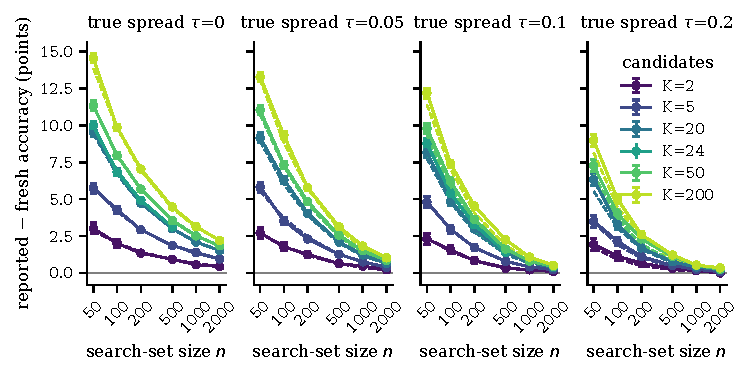
\includegraphics[width=\linewidth]{fig_a_optimism.pdf}
\caption{\textbf{Optimism of the naive report in the synthetic world (T0).} Reported minus fresh-item accuracy of the selected configuration against search-set size $n$, for $K$ candidates searched exhaustively, one panel per true spread $\tau$. Points: mean over 1000 replicates per cell, bars: 95\% CI; dashed: extreme-value prediction. Reference world $\rho=0.6$, baseline accuracy 0.3.}
\label{fig:A}
\end{figure}
\begin{figure}[t]
\centering
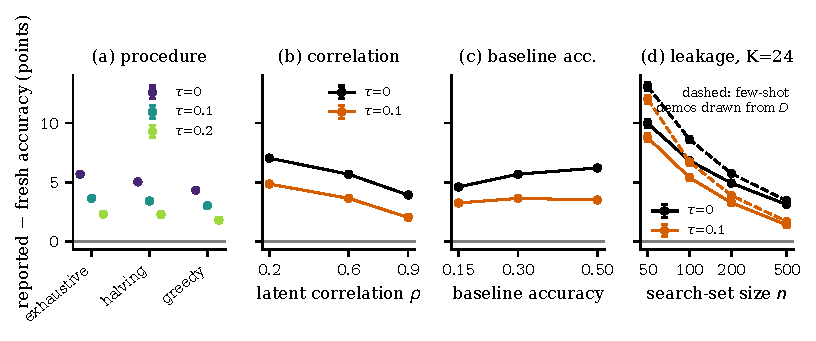
\includegraphics[width=\linewidth]{fig_b_factors.pdf}
\caption{\textbf{Other drivers of optimism (T0).} Same quantity; $n=200$, $K=50$ unless stated. (a) search procedure, (b) correlation $\rho$ between configurations' item outcomes, (c) baseline accuracy, (d) few-shot demonstrations drawn from $D$ (dashed) or not, $K=24$. 1000 replicates per point.}
\label{fig:B}
\end{figure}

\textbf{Does it change conclusions?} (Tables~\ref{tab:D},~\ref{tab:E}.) Take the claim ``tuned beats the untuned baseline by more than $m=2$ points'' with $K=200$, $n=100$. When the truth is $\tau=0$ (no gain), the naive point comparison claims it 97.6 [96.5, 98.4]\% of the time. Comparing two tuned systems on reported scores, the system searched over $K=200$ candidates is declared better than one searched over $K=5$ in 86.7 [84.5, 88.7]\% of replicates although they are equal, and a system tuned on $n=50$ items beats one tuned on $n=500$ in 93.2 [91.5, 94.6]\% of replicates ($K=50$). The reported ranking thus tracks search effort and set size rather than quality.

\subsection{Reporting methods: calibration and decisions (T0)}
\textbf{Targets and metrics.} Each method reports an estimate and, where available, a nominal 95\% interval for $\theta(\hatc)$ (M2: for the expected fresh accuracy of the fold-selected configurations). We measure bias, RMSE, coverage, width and the number of items consumed (Table~\ref{tab:C}, Fig.~\ref{fig:C}).

\begin{figure}[t]
\centering
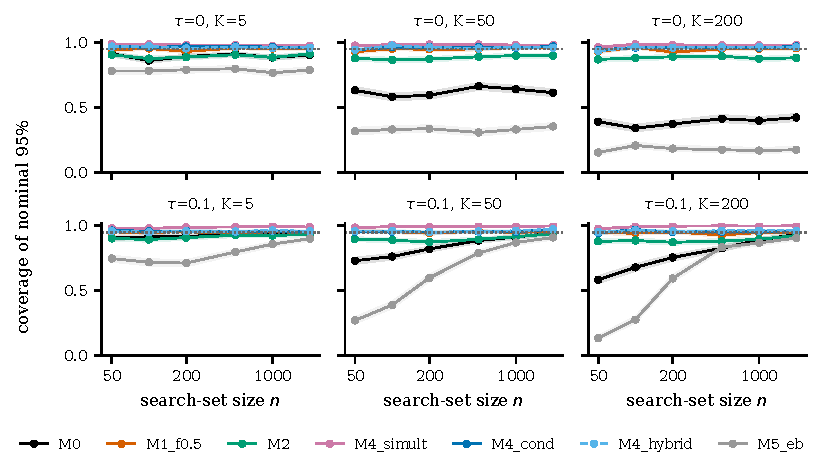
\includegraphics[width=\linewidth]{fig_c_coverage.pdf}
\caption{\textbf{Coverage of nominal-95\% intervals (T0).} Wilson 95\% bands over 1000 replicates; dotted: 0.95. M0: same-set interval; M1\_f0.5: hold-out with half of $D$ for selection; M2: 5-fold cross-fitting; M4\_simult: simultaneous max-type bound; M4\_cond, M4\_hybrid: conditional/hybrid selection-aware intervals; M5\_eb: empirical Bayes from disclosed scores.}
\label{fig:C}
\end{figure}

\begin{table}[t]
\caption{\textbf{Calibration of reporting methods (T0), $K=200$, $n=100$, 1000 replicates per cell} ($n=500$ and the other methods in the appendix, Table~\ref{tab:Cfull}). Bias and RMSE in accuracy points; coverage with Wilson 95\% interval; width in points; items used for the report. Ladder/optimism-corrected point reports have no interval and appear in the appendix.}
\label{tab:C}
\centering\scriptsize
\resizebox{\linewidth}{!}{\begin{tabular}{llrrrrrr}
\toprule
$\tau$ & $n$ & method & bias (pts) & RMSE (pts) & coverage [Wilson 95\%] & width (pts) & items for report \\
\midrule
0 & 100 & M0 & +9.85 $\pm$ 0.21 & 10.40 & 0.341 [0.312, 0.371] & 18.9 & 100 \\
0 & 100 & M1\_f0.5 & -0.08 $\pm$ 0.40 & 6.38 & 0.964 [0.951, 0.974] & 24.6 & 50 \\
0 & 100 & M2 & -0.03 $\pm$ 0.34 & 5.49 & 0.880 [0.858, 0.899] & 17.7 & 100 \\
0 & 100 & M4\_simult & +9.85 $\pm$ 0.21 & 10.40 & 0.986 [0.977, 0.992] & 34.2 & 100 \\
0 & 100 & M4\_cond & -3.99 $\pm$ 1.86 & 30.22 & 0.961 [0.947, 0.971] & 45.8 & 100 \\
0 & 100 & M4\_hybrid & +2.61 $\pm$ 0.46 & 7.94 & 0.964 [0.951, 0.974] & 27.3 & 100 \\
0 & 100 & M5\_eb & -0.09 $\pm$ 0.17 & 2.81 & 0.208 [0.184, 0.234] & 1.3 & 100 \\
0 & 100 & M5\_ladder & -1.17 $\pm$ 0.63 & 10.26 & -- & -- & 100 \\
\midrule
0.1 & 100 & M0 & +7.40 $\pm$ 0.25 & 8.40 & 0.680 [0.650, 0.708] & 19.1 & 100 \\
0.1 & 100 & M1\_f0.5 & -0.29 $\pm$ 0.42 & 6.73 & 0.943 [0.927, 0.956] & 25.4 & 50 \\
0.1 & 100 & M2 & -0.35 $\pm$ 0.37 & 5.90 & 0.886 [0.865, 0.904] & 18.4 & 100 \\
0.1 & 100 & M4\_simult & +7.40 $\pm$ 0.25 & 8.40 & 0.993 [0.986, 0.997] & 34.6 & 100 \\
0.1 & 100 & M4\_cond & -3.21 $\pm$ 1.44 & 23.42 & 0.970 [0.957, 0.979] & 41.5 & 100 \\
0.1 & 100 & M4\_hybrid & +1.34 $\pm$ 0.46 & 7.52 & 0.964 [0.951, 0.974] & 27.5 & 100 \\
0.1 & 100 & M5\_eb & -4.67 $\pm$ 0.24 & 6.05 & 0.278 [0.251, 0.307] & 5.3 & 100 \\
0.1 & 100 & M5\_ladder & -1.48 $\pm$ 0.63 & 10.20 & -- & -- & 100 \\
\bottomrule
\end{tabular}
}
\end{table}

\textbf{Findings (T0, $K=200$, $\tau=0$, $n=100$; Table~\ref{tab:C}).} The naive interval covers $\theta(\hatc)$ in only 34.1 [31.2, 37.1]\% of replicates (bias $+9.85\pm0.21$ points); even at $n=500$ coverage is 41.4\%, and at $\tau=0.1$ it is 68.0\% and 82.7\% at $n=100$ and $500$. (i) \emph{Hold-out} (M1) is unbiased and covers at the nominal level (0.96 for all three split fractions), but it pays in items and width: 19.7 to 37.3 points wide at $n=100$ and, with half of $D$ held out, RMSE 6.4 vs.\ 10.4 points for M0. (ii) \emph{Cross-fitting} (M2) is unbiased for the expected fresh accuracy of the procedure's selections but its interval undercovers (0.88 [0.86, 0.90]; 0.86--0.95 over the 128 reference cells), because fold scores are dependent. (iii) \emph{Selection-aware inference} (M4): the simultaneous bound covers (0.986) but is as biased as M0 and wide (34.2 points); the conditional (0.961) and hybrid (0.964, width 27.3 points) intervals reach nominal coverage (0.94--0.98 over the 128 reference cells, as for M1\_f0.5 at 0.92--0.97), but the conditional point estimate is heavy-tailed (RMSE 30 points at $n=100$) so only its interval is usable, and hybrid has bias $+2.6$ points. (iv) Bootstrap optimism correction (M3) removes only part of the bias ($+1.9$ points for $n=200$; $+2.5$ for the .632 variant, vs.\ $+7.0$ for M0; appendix). (v) The empirical-Bayes interval from the disclosed scores (M5\_eb) fails: coverage 0.21 at $\tau=0$, $K=200$, $n=100$, and 0.09--0.93 across the 128 reference cells (Fig.~\ref{fig:C}), since candidates share items; we report it as a negative result. The Ladder-style report has no interval; its point report is $-1.2\pm0.6$ points biased with step $n^{-1/3}$ but $+8.2\pm0.3$ with the $0.5/\sqrt n$ step, i.e.\ its calibration depends on a free step size.

\begin{table}[t]
\caption{\textbf{False-claim rate and power of ``tuned beats baseline by $>2$ points'' (\%, Wilson 95\%), $K=200$, $n=100$ (T0).} ``point'': estimate difference exceeds $m$; ``lower bound'': the method's 95\% lower bound exceeds the baseline's estimate $+m$. At $\tau=0$ the true gain is 0. At $\tau=0.1$, 162 false-claim and 608 power replicates (per-cell counts in \texttt{tables/table\_d\_all\_cells.csv}).}
\label{tab:D}
\centering\scriptsize
\resizebox{\linewidth}{!}{\input{../tables/table_d_decisions.tex}}
\end{table}

\textbf{Decisions (Table~\ref{tab:D}).} Naive reports make a false improvement claim in 97.6\% of replicates when there is no improvement; using the naive lower bound this is still 38.4 [35.4, 41.5]\%. Hold-out, cross-fitting and the selection-aware lower bounds bring the false-claim rate to 0.5--4.1\% with a lower-bound rule, but at this sample size the price is power: at $\tau=0.1$ the power to detect a true gain of $\geq 2$ points falls from 73.7 [70.6, 76.6]\% (naive lower bound, which is not valid) to 10.8--27.4\% (valid rules). The point-comparison rule has a high false-claim rate even for unbiased methods (32--43\% for M1/M2) because the difference of two noisy scores exceeds $m=2$ points by chance; \emph{unbiasedness does not by itself license a claim}.
\subsection{Real LLM on real MMLU-Pro (T1)}
\label{sec:t1}
\textbf{Design.} The system is Qwen2.5-1.5B-Instruct~\citep{qwen2024qwen25} (Q8\_0 GGUF, llama.cpp, CPU; Apache-2.0) answering MMLU-Pro~\citep{wang2024mmlupro} (pinned revision, MIT license, 10 options) by reading out the log-probabilities of the ten option letters. The configuration family has 24 base prompts (4 instruction styles $\times$ 2 answer cues $\times$ \{0-shot, two 3-shot demonstration sets from the validation split\}) plus the 276 two-prompt logit-average ensembles of them as a pipeline-like extension: $K_{\max}=300$ candidates. All 300 are scored once on a fixed pool of 2000 randomly drawn test questions and the per-item outcomes are cached; a search is then \emph{replayed}: draw a search set $D$ of $n$ pool items, let the procedure choose $\hatc$ among $K$ candidates (the baseline prompt plus $K-1$ random ones; $K=24$ is the base family), and score $\hatc$ on the remaining pool items minus a left-out block (1300--1750 fresh items, binomial SE $\approx$1.1--1.3 points, independent of the search). The pool accuracies of the 24 base prompts range from 20.5\% to 29.2\% and the best of all 300 is 30.1\%; the between-candidate spread is small ($\tau\approx0.017$--$0.024$ on the probability scale) and candidates are strongly correlated (binary item correlation 0.57--0.68). The baseline prompt has 22.7\%. 52 replay cells with 1000 replicates each; because replicates share the fixed pool, every uncertainty in this subsection is $\pm1.96\times$ a delete-a-block SE (10 blocks of replicates) rather than a replicate SE or Wilson interval; it reflects the variation over search sets given the pool, not the uncertainty about the pool itself, which we do not estimate.

\textbf{Gap.} (Fig.~\ref{fig:A1}.) The naive report is optimistic here too. For $K=300$ and $n=100$ the selected configuration is reported at 33.7\% and scores 28.0\% on fresh items: a 5.7-point gap (block SE 0.11). Against the baseline's 22.7\%, the reported improvement is 11.0 points while the real one is 5.3: about twice as large. The gap is 8.7 points at $n=50$ and 1.9 at $n=500$ ($K=300$), and 4.6 points for the 24 base prompts alone ($n=100$). It grows with $K$ and falls with $n$ like the extreme-value formula evaluated with the matrix's own $(\sigma,r,\tau)$, which is within 0.51 points of every one of the 35 exhaustive cells (mean difference $-0.04$ points), although 13 of the 35 differ by more than 1.96 block SE, mostly at small $K$ and $n=50$ where it over-predicts (e.g.\ $K=2$, $n=50$: 1.80 predicted, 1.29 observed). The parameters are estimated from the same matrix, so this checks the functional form, not a held-out prediction. The synthetic grid of T0 gives a larger gap than the real one in 28 of its 30 nearest cells (median ratio 1.6; its correlation grid does not contain the matrix's), so we treat T0 as a model of the mechanism, not a calibrated replica (Fig.~\ref{fig:T1check}, appendix). Halving and greedy search are mildly less optimistic than exhaustive search (4.0 and 4.1 vs.\ 4.5 points at $n=100$, $K=24$; 5.2 vs.\ 5.7 at $K=300$). The gap is present in every one of the 14 MMLU-Pro subjects (3.3 to 7.0 points at $n=100$, $K=24$; Fig.~\ref{fig:T1subj}, appendix).

\textbf{Reporting methods and decisions.} (Table~\ref{tab:G}.) The naive interval covers $\theta(\hatc)$ in 77.1 $\pm$ 3.2\% ($n=100$) and 80.6 $\pm$ 2.2\% ($n=500$; $\pm1.96$ block SE) of replicates at $K=300$ and is biased by $+5.7$ and $+1.9$ points. Hold-out (M1, 0.95/0.94 at half split), the hybrid conditional interval (0.953/0.935) and cross-fitting (0.92/0.88) are close to nominal and unbiased; the conditional interval is nominal but its point estimate is heavy-tailed (RMSE 20.8 points at $n=100$); the simultaneous bound is conservative (0.988) and as biased as M0; the empirical-Bayes interval again fails (0.11/0.22). Bootstrap optimism correction removes most but not all of the bias ($+1.8$ points at $n=100$, $K=300$, vs.\ $+5.7$ for M0; appendix). Because the 276 ensembles are not independent systems and the candidates differ little, "tuned beats baseline" is almost always true here, so false-claim rates are not identifiable from these cells; we use a paired design instead (Table~\ref{tab:H}): two systems tuned with $K_A=75$ and $K_B=5$ candidates on the same $n=100$ items, where the true difference is on average 0.5 points and A is truly better in only 61.7\% of the replicates. Naive reports declare A better in 90.3\% of replicates (the reported difference is $+3.0$ points against a true $+0.5$); among the 383 replicates in which A is not truly better, 87.5\% still call it better with M0, versus 43--56\% for hold-out, cross-fitting and the selection-aware point rules. With a rule that requires A's 95\% lower bound to exceed B's estimate the false-winner rate is 0\% for M0 and the simultaneous bound and 3.1--3.4\% for hold-out, cross-fitting and the conditional/hybrid intervals, but those rules detect a truly better A in only 7--9\% of replicates (M0: 1.8\%); the equal-$K$ pairs have no true difference, and every report order there is a coin flip (flip rates near 0.5 by construction).

\begin{figure}[t]
\centering
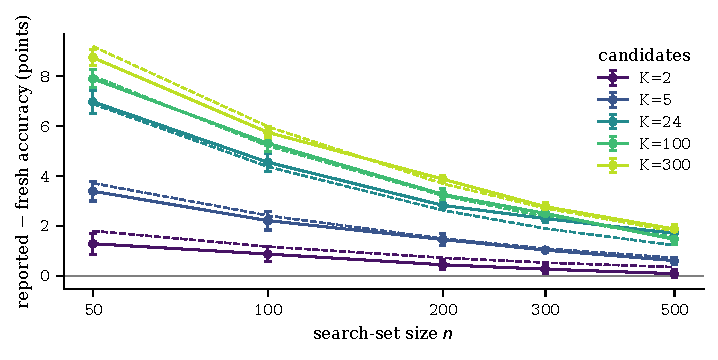
\includegraphics[width=\linewidth]{fig_a_t1.pdf}
\caption{\textbf{Optimism of the naive report on the real outcome matrix (T1).} Reported minus fresh-item accuracy of the selected configuration against $n$, for $K$ candidates searched exhaustively (Qwen2.5-1.5B-Instruct, MMLU-Pro; 1000 replicates per cell). Bars: mean $\pm1.96\times$ delete-a-block SE (replicates share one 2000-item pool, so the replicate SE is too small); dashed: the closed form fed with the matrix's own $(\sigma,r,\tau)$.}
\label{fig:A1}
\end{figure}

\begin{table}[t]
\caption{\textbf{Calibration of reporting methods on the real matrix (T1), $K=300$, $n=100$, 1000 replicates} ($n=500$ in the appendix). Bias and RMSE in points against each method's own target; coverage $\pm1.96$ block SE; median width (points); items used for the report.}
\label{tab:G}
\centering\scriptsize
\resizebox{\linewidth}{!}{\input{../tables/table_g_main.tex}}
\end{table}

\begin{table}[t]
\caption{\textbf{Ranking two tuned systems on the same search set (T1).} A and B are tuned exhaustively from disjoint candidate subsets of $K_A$ and $K_B$ configurations; 1000 replicates per cell, $\pm1.96$ block SE. Flip: the reported order differs from the true order (a tie counts as a flip). The 75 vs.\ 5 pair has the largest search-effort contrast; the equal-$K$ pairs are controls with no true difference.}
\label{tab:H}
\centering\scriptsize
\resizebox{\linewidth}{!}{\input{../tables/table_h_t1_pairs.tex}}
\end{table}

